
\section*{Exercice 1 -- Construction d'une pile}
On souhaite réaliser les fonctions de base permettant la gestion d'une pile. On souhaite que celle-ci soit implémentée sous la forme d'une liste. La taille de la pile doit être limitée à \texttt{n} données.

Ainsi, une pile de taille 5 avec 4 éléments sera de la forme suivante : \texttt{[1,2,3,4,None]}.

\subparagraph{}\textit{Implémenter la fonction \texttt{creer\_pile(n)} permettant de créer une pile de taille n.  Les spécifications seront les suivantes :}
\begin{py}
\begin{python}
def creer_pile(n):
    """
    Créer une pile de taille n.
    Entrée : 
     * n(int) : taille souhaitée de la pile
    Sortie : 
     * pile(list) : pile de taille n.
     sinon
    """
\end{python}
\end{py}

\subparagraph{}\textit{Implémenter la fonction \texttt{est\_vide} permettant de vérifier qu'une pile est vide. Les spécifications de la fonction seront les suivantes : }
\begin{py}
\begin{python}
def est_vide(pile):
    """
    Vérifie si la pile est vide.
    Entrée : 
     * pile(list)
    Sortie : 
     * retourne True si la pile est vide, False 
     sinon
    """
\end{python}
\end{py}
\subparagraph{}\textit{Implémenter la fonction \texttt{est\_pleine} permettant de vérifier qu'une pile est pleine. Les spécifications de la fonction seront les suivantes :}
\begin{py}
\begin{python}
def est_pleine(pile,nb):
    """
    Vérifie si la pile est pleine.
    Entrée : 
     * pile(list)
     * nb(int) : nombre d'éléments maximum dans une pile
    Sortie : 
     * retourne True si la pile est pleine, False 
     sinon
    """
\end{python}
\end{py}
\subparagraph{}\textit{Créer la fonction \texttt{empiler} permettant d'ajouter un élément au sommet de la pile. Les spécifications de la fonction devront être indiquées.}

\subparagraph{}\textit{Créer la fonction \texttt{depiler} permettant de supprimer l'élément au sommet de la pile et de le renvoyer. Les spécifications de la fonction devront être indiquées.}

\subparagraph{}\textit{Créer la fonction \texttt{taille\_pile} permettant de donner la longueur de la pile.}




\section*{Exercice 2}

Écrire une fonction concaténant deux piles. \\
Cette fonction prendra en argument deux piles et placera la première << sur >> la deuxième. Elle ne renverra rien, mais 
modifiera les deux piles : à la fin, la première pile sera vide et la seconde aura été augmentée de la première. Pour 
cela, on supposera que la seconde pile est assez grande pour recevoir toute la première.

On proposera une version itérative et récursive.
\ifprof
\section*{Corrigé 1}
\begin{python}
def concat (P1,P2) :
    if est_vide(P1) :
	return None
    else :
	x = depiler(P1)
	concat(P1,P2)
	empiler(P2,x)
\end{python} 
\else
\fi

\section*{Exercice 3}

Écrire une fonction renvoyant la plus grande somme possible de trois éléments consécutifs d'une pile d'entiers 
naturels. Si la pile a deux éléments ou moins, on renverra 0. On prendra garde de recopier la pile passée en argument 
afin de ne pas la modifier.

\ifprof
\section*{Corrigé 3}

\begin{python}
def somme3 (P) :
    R = P.copy()
    if est_vide(R) :
	return 0
    else :
	x = depiler(R)
	s = somme3(R)
	for i in range(2) :
	if est_vide(R) :
	    return s
	else :
	    x += depiler(R)
	return max(x,s)
	    
\end{python} 


\else \fi
\section*{Exercice 4}

On se donne deux piles $P_1$ et $P_2$, et on se propose de fusionner ces deux piles en une seule pile $P$ de manière 
à respecter les règles suivantes :
\begin{enumerate}
\item Si $P_1=[a_1,a_2,\cdots,a_{n-1},a_n]$ et $P_2=[b_1,b_2,\cdots,b_{p-1},b_p]$, alors 
$P=[\cdots,b_{p-1},a_{n-1},b_p,a_n]$.
\item Si l'une des pilees est vide, alors on n'a plus recours qu'à l'autre, jusqu'à ce que celle-ci aussi soit vide.
\end{enumerate}
Exemples : $P_1=(a_1,a_2,a_3)$ et $P_2=(b_1,b_2,b_3,b_4,b_5)$, alors $P=[b_1,b_2,a_1,b_3,a_2,b_4,a_3,b_5]$.\\

Écrire une fonction python réalisant cela. On prendra garde de recopier les piles passées en argument afin de ne pas la 
modifier.\\
Afin d'être sûr que la nouvelle pile est assez grande pour contenir les deux premières, on pourra commencer par écrire 
une fonction recopiant une pile dans une autre pile de taille donnée.

\ifprof

\section*{Corrigé 4}


\begin{python}
def copie (P,n) :
    """ recopie la pile P dans une pile de taille n.
    préconditon : n > taille_pile(P) """
    l = taille_pile(P)
    R = P.copy()
    assert n>l
    if est_vide(R) :
        return creer_pile(n)
    else :
        x = depiler(R)
        S=copie(R,n)
        empiler(S,x)
        return S

def fusion (P1,P2) :
    n = taille_pile(P1)+taille_pile(P2)
    R1 = P1.copy()
    R2 = P2.copy()
    if est_vide(R1) :
        return copie(R2,n)
    if est_vide(R2) :
        return copie(R1,n)
    else :        
        e1 = depiler(R1)
        e2 = depiler(R2)
        R3 = fusion(R1,R2)
        empiler(R3,e1)
        empiler(R3,e2)
        return R3 
\end{python} 
\else \fi



\section*{Exercice 5 -- Notation polonaise inversée}
\setcounter{exo}{0}
La notation polonaise inversée permet de réaliser des opérations arithmétiques sans utiliser de parenthèses. On parle aussi d'expressions \textbf{postfixées}. Dans cette notation, l'opérateur (+, -, *, /) suit toujours l'opérande (nombres). Ici, l'opération suit le deuxième opérande.

On doit évaluer une expression composée d'opérateurs et d'opérandes. L'expression est lue de gauche à droite en suivant les règles suivantes :
\begin{itemize}
\item si on lit une opérande, on l'empile;
\item si on lit un opérateur, on dépile deux opérandes, on réalise le calcul et on empile le résultat. 
\end{itemize}
\begin{exemple}
Pour calculer $7\cdot 2$, on évalue l'expression $7\;2\; *$.

Pour calculer $((1 + 2) \cdot 4) + 3$, on évalue l'expression $1\;2\;+\;4\;*\;3\;+$.
\end{exemple} 


\begin{rem}
Le principal avantage de cette méthode est la suppression totale des parenthèses. En contrepartie, elle nécessite une petite gymnastique intellectuelle pour les néophytes que nous sommes.

Cette notation est utilisée dans certaines calculatrices HP et dans certains utilitaires (programme calc d'Emacs, description des bibliographies dans LaTeX \textit{etc.}).
\end{rem}

Dans cet exercice, la pile sera implémentée sous forme d'une liste d'opérande et d'opérateurs. 

\textbf{On utilisera les fonctions définies à l'exercice précédent.}
 
\subparagraph{}\textit{Créer la fonction \texttt{est\_nombre} permettant de savoir si une variable est un nombre ou non.}

\subparagraph{}\textit{Créer la fonction \texttt{est\_operation} permettant de savoir si une variable est une opération ou non.}

\subparagraph{}\textit{L'expression postfixée se lisant de gauche à droite et les outils permettant de traiter la pile traitant cette dernière de droite à gauche, réaliser la fonction \texttt{inversion} permettant d'inverser les éléments de la pile.}


\subparagraph{}\textit{Créer la fonction \texttt{evaluer} permettant d'évaluer une expression postfixée. Les spécifications sont les suivantes :}

\begin{py}
\begin{python}
def evaluer(exp):
    """
    Évaluer le résultat d'une opération post-fixée.
    Entrée : 
     * ex(lst) : liste d'opérateurs et d'opérandes
    Sortie : 
     * res(flt) : résultat du calcul de l'expression.
    """
\end{python}
\end{py}

\subparagraph{}
\textit{Transcrire l'expression suivante en NPI puis l'évaluer : $5+\left(\left( 1+2\right)\times4 \right)-3$.}
%
%\section*{Exercice 3 -- Croisement routier}
%\setcounter{exo}{0}
%\textit{D'après P. Beynet.}
%
%Pour simuler un croisement routier, à sens unique, on utilise 3 files \texttt{f1}, \texttt{f2} et \texttt{f3} représentant respectivement les voitures arrivant sur des routes \texttt{f1} et \texttt{R2}, et les voitures partant sur la route \texttt{R3}.
%La route \texttt{R2} a un STOP. Les voitures de la file \texttt{f2} ne peuvent avancer que s’il n’y a aucune voiture sur la route \texttt{R1}, donc dans la file \texttt{f1}. On souhaite écrire un algorithme qui simule le départ des voitures sur la route \texttt{R3}, modélisée par la file \texttt{f3}.
%\begin{center}
%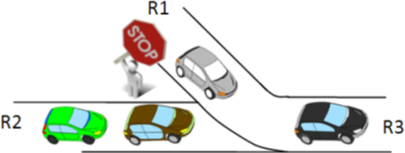
\includegraphics[width=.8\linewidth]{images/file_01}
%\end{center}
%On utilise trois files \texttt{f1}, \texttt{f2} et \texttt{f3} de valeurs booléennes :
%\begin{itemize}
%\item  « 1 » symbolise la présence d’une voiture;
%\item  « 0 » l’absence de véhicule.
%\end{itemize}
%
%\subparagraph{}
%\textit{Réaliser l'algorithme de croisement routier permettant de simuler la composition de la file \texttt{f3} en fonction de la composition des files \texttt{f1} et \texttt{f2}. Les files seront modélisées par des listes de booléens.}
